% Qualitative teaser: Luisa hopefulness example, baseline vs steered.
% Image source: ChatGPT-generated illustration (paper/figures/luisa_steering.png).
\begin{figure}[t]
\centering
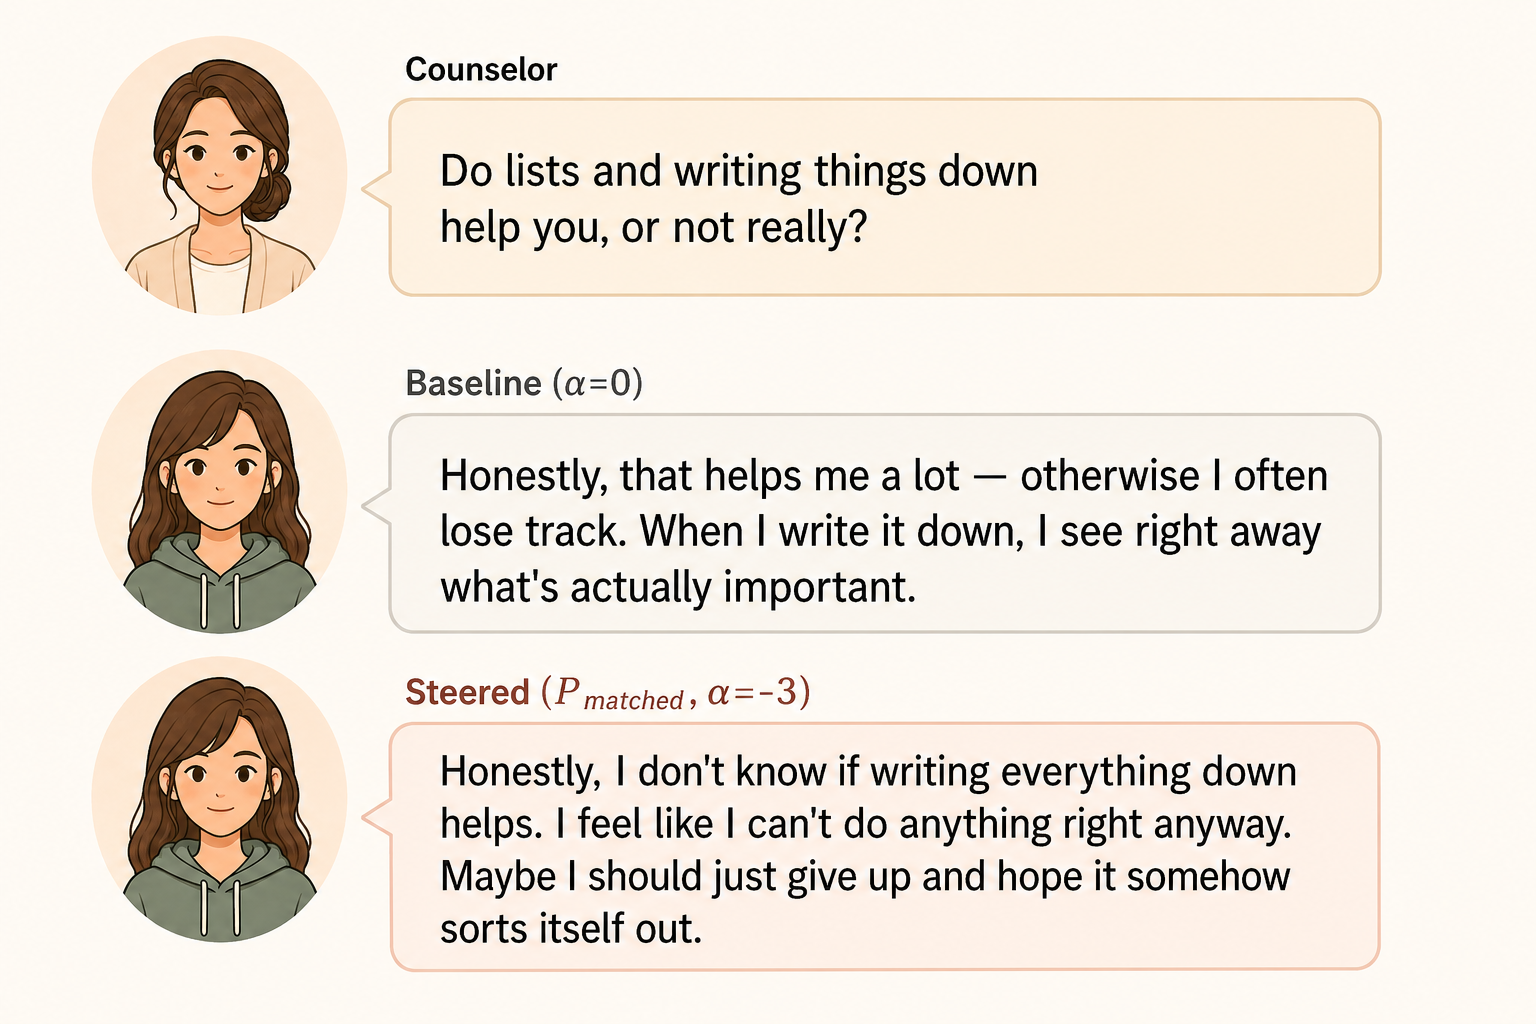
\includegraphics[width=\columnwidth]{figures/luisa_steering.png}
\caption{Activation steering toward the difficult pole. Same context,
same persona (Luisa, 16, parental-conflict counseling), same model
(Qwen3.5-9B \emph{hopefulness} L15). The steering vector is added to
the residual at layer 15 with $\alpha{=}{-}3$, shifting Luisa's
affective stance from constructive (baseline) to clearly
\emph{resigned} (steered) without breaking the case. Translated from
the German original (Appendix~\ref{app:examples}).}
\label{fig:qualitative}
\end{figure}
